\documentclass[a4paper,12pt,article]{memoir}
\usepackage{amsmath}
\usepackage{amssymb}
\usepackage{mathspec}
\usepackage{xltxtra}
\usepackage{polyglossia}
\usepackage{MnSymbol}
\usepackage{siunitx,cancel,graphicx}
\usepackage{enumitem}
\usepackage{hyperref,graphicx}
\usepackage{icomma}
\usepackage{float}
\usepackage{mleftright}

\usepackage{listings}
\usepackage{color}
\usepackage{xcolor}

\usepackage[
backend=biber,
style=numeric,
citestyle=numeric,
sorting=none
]{biblatex}
\addbibresource{resources.bib}


% This is the color used for MATLAB comments below
\definecolor{MyDarkGreen}{rgb}{0.0,0.4,0.0}
\definecolor{Blue}{rgb}{0.0,0.0,1.0}
\definecolor{Purple}{rgb}{1.0,0.0,1.0}

\colorlet{mygray}{black!30}
\colorlet{mygreen}{green!60!blue}
\colorlet{mymauve}{red!60!blue}

\lstset{
  backgroundcolor=\color{gray!10},
  basicstyle=\ttfamily,
  columns=fullflexible,
  breakatwhitespace=false,
  breaklines=true,
  captionpos=b,
  commentstyle=\color{mygreen},
  extendedchars=true,
  frame=single,
  keepspaces=true,
  keywordstyle=\color{blue},
  language=c++,
  numbers=none,
  numbersep=5pt,
  numberstyle=\tiny\color{blue},
  rulecolor=\color{mygray},
  showspaces=false,
  showtabs=false,
  stepnumber=5,
  stringstyle=\color{mymauve},
  tabsize=3,
  title=\lstname
}






\setdefaultlanguage{english}

\defaultfontfeatures{Scale=MatchLowercase,Mapping=tex-text}
%\setmainfont[Numbers=Lowercase]{Minion Pro}
%\setsansfont[Numbers=Lowercase]{Myriad Pro}
%\setmonofont{Menlo}
%\setmathsfont(Digits,Latin,Greek)[Numbers={Lining,Proportional}]{Minion Pro}

\sisetup{%
  output-decimal-marker = {,},
  per-mode = symbol,
  %round-mode = places,
  %round-precision = 5
}



\setlrmarginsandblock{2.5cm}{2.5cm}{*}
\setulmarginsandblock{1.5cm}{2cm}{*}
\checkandfixthelayout

\setlength{\parindent}{2em}
\setlength{\parskip}{0pt}

\newcommand{\f}{\fancybreak}

\DeclareSIUnit \electronvolt {\ensuremath{eV}}
\DeclareSIUnit \lightspeed {\ensuremath{c}}
\DeclareSIUnit \dalton{\ensuremath{u}}
\DeclareSIUnit \echarge{\ensuremath{e}}


\newcommand{\mvec}[2]{
\ensuremath{\left(
\begin{array}{c}
#1\\
#2\\
\end{array}
\right)}
}

\newcommand{\Span}{\ensuremath{\mathrm{Span}}}
\newcommand{\Mat}{\ensuremath{\mathrm{Mat}}}
\newcommand{\C}{\ensuremath{\mathbb{C}}}
\newcommand{\R}{\ensuremath{\mathbb{R}}}
\newcommand{\Rno}{\ensuremath{\mathbb{R}\backslash\{0\}}}
\newcommand{\Z}{\ensuremath{\mathbb{Z}}}
\newcommand{\ol}[1]{\ensuremath{\overline{#1} } }
\newcommand{\F}[1]{\ensuremath{\mathbb{F}_{#1} } }

\title{Student Colloquium, Simulating particles in a solenoids}
\author{Nikolaj Roager Christensen}
\date{\today} %

\begin{document}

\maketitle


\tableofcontents*

\chapter{Progress this week}
This week, I applied my simulation to particles traveling in a straight or curved solenoid.

I also made some updates to how the data is displayed (particle path includes time-stamp points and names, and I also draw visual aides, in this case rings, to indicate the solenoid).

\chapter{Particles in a solenoid}
The magnetic field of a straight solenoid is as simple as it is possible to be.

If a solenoid has $n$ turns of wire per unit length, where each wire carries current $I$, and the solenoid is wrapped counterclockwise around the $\vec{\hat{n}}$ with radius $R$, as on figure \ref{fig:sol0}, then the field a distance $r$ from the center is\

\begin{equation}
\vec{B}(r)=\vec{\hat{n}}\begin{cases}\mu_0 I n & r<R\\0 &r>R \end{cases}.
\end{equation}

This can be shown using Ampere's law, as illustrated on figure \ref{fig:sol0}. Ampere's law states that the field around the loops $A$ and $B$ is $\oint B \cdot d\vec{l} = \mu_0 I_{encl}$. here the current through loop $A$ is $I_{encl,A}=n l I$ and the current through loop $B$ is $0$. Alongside the symmetry of the setup, this allows us to find the field.


\begin{figure}
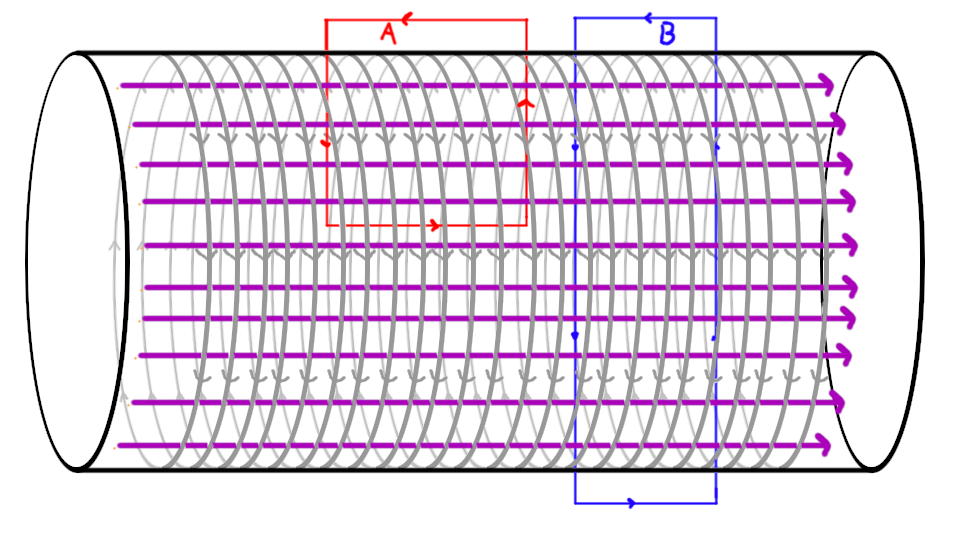
\includegraphics[width=\linewidth]{solenoid.png}
\caption{Sketch of a solenoid (black), with 2 imaginary loops (red and blue), which can be used to calculate the field (purple).}
\label{fig:sol0}
\end{figure}

\section{Simulation setup and units}
This field is easy to set up in the simulation, and in the first example I use a solenoid along the x-axis with 1000 turns per meter, with a current of \SI{5}{\ampere} and a radius of \SI{0.6}{\meter} (for reasons which will become apparent later). This gives us a field inside the solenoid:


\begin{equation}
\vec{B}_{inside} \approx\vec{x} \SI{6.28}{\milli\tesla}.
\end{equation}
%0.006283185307179587 T


In the simulation, I will look at a proton, with charge $q_p=e=\SI{1.60E-19}{\coulomb}$ and mass $m_p=\SI{1.67E-27}{\kilo\gram}$.



Regardless of the velocity of the particle the ``cyclotron frequency" is:

\begin{equation}
\omega = \frac{q_p B}{m_p} \approx \SI{6.02E5}{\hertz}
\end{equation}
%601855.8374534972 Hz

so a particle will make one full rotation each $1/\omega \approx \SI{1.66E-05}{\second}$.


Then we should pick what velocity the particle in the simulation is traveling at, let us for instance say we have a particle with a kinetic energy of  $\SI{1}{\mega\electronvolt\per\square\lightspeed}$, sticking with classical physics for now, that equates to $|v|=\SI{3.195E5}{\meter\per\second}$ (still so much less than the speed of light I do feel comfortable using non-relativistic physics). We know that the Cyclotron  radius (aka. Larmor-, or gyroradius ) , i.e. the radius of the cyclotron path is  $r_c= m_p v_\perp/Bq_p$. So if a particle with this velocity is traveling entirely perpendicular to the field it will trace out a circle with radius:

%319515.54756336455 m/s
\begin{equation}
r_c = \frac{m_p v_\perp}{B q_p} \approx \SI{0.531}{\meter}
\end{equation}
%0.5308837466149273 r
%1.661527458520772e-06 s

Hence why I picked the radius of the Solenoid to be \SI{0.6}{\meter}.

The precision of \lstinline{double} in C++ is $2^{-53}\approx 10^{-15}$ (on my computer at least, specified as \lstinline{DBL_MANT_DIG} in \lstinline{float.h}). So as far as the simulation is concerned $q_p=0$ and $m_p=0$.

One option is to use arbitrary precision floating point numbers (e.g. \cite{arb}), which have potentially infinite precision, at the cost of having undefined data size. However that would make it harder to save and load data as binary.

Instead, I just pick our base time, mass, charge and distance unit to be around 1 at the scales we are working with, I choose, micro-seconds, atomic mass units, elementary charge (obviously) and meters. Under this system, the relevant characteristics are roughly (the constants and conversions are used with higher precision than shown here):

\begin{table}
\begin{tabular}{c @{\quad} c @{\quad} c}
\toprule
Variable           & SI units                        & Simulation units\\
\midrule
$ \si{\kilo\gram}$ & \SI{1}{\kilo\gram}              & \SI{6.022E26}{\dalton}\\ %6.02214076
$ \si{\coulomb}$   & \SI{1}{\coulomb}                & \SI{6.242E18}{\echarge}\\%6.242
$ \si{\second}$    & \SI{1}{\second}                 & \SI{1E6}{\micro\second}\\
$ \si{\tesla}$     & \SI{1}{\kilo\gram\per\second\per\coulomb}&\SI{96.49}{\dalton\per\micro\second\per\echarge}\\ %96.4853322
\midrule
$m_p$              & \SI{1.67E-27}{\kilo\gram}                      & \SI{1.01}{\dalton}\\
$q_p$              & \SI{1.60E-19}{\coulomb}                        & \SI{1.0}{\echarge}\\
$v$                & \SI{3.20E5}{\meter\per\second}                & \SI{0.32}{\meter\per\micro\second}\\
%$\mu_0$            & \SI{1.26E-6}{\newton\per\square\ampere}        & \SI{1.94E-17}{\dalton\meter\per\square\echarge}\\
$\vec{B}_{inside}$ & $\vec{x} \SI{6.28}{\milli\tesla}$              & $\vec{x}\SI{0.61}{\dalton\per\micro\second\per\echarge}$\\
$\omega$           & \SI{6.02E5}{\per\second}                       & \SI{0.602}{\per\micro\second}\\
$r_c$              & \SI{0.53}{\meter}                              & \SI{0.53}{\meter}\\
\bottomrule
\end{tabular}
\caption{Variables used in simulation in SI units and in the units used internally in the simulation}
\label{tab:units}
\end{table}

\section{Particles in a Solenoid}
The first experiment, which is mostly a proof that the unit conversion has worked is a proton with kinetic energy $\SI{1}{\mega\electronvolt\per\square\lightspeed}$ in the solenoid setup in the previous section, traveling at an angle $ \ang{0} \leq\theta\leq \ang{90}$ in steps of $\ang{15}$ relative to the x-axis (the direction of the solenoid), the particles are offset by their cyclotron radius from the center of the solenoid.

As we already know, a 3D plot including the particle path and the magnetic field is not particularly readable, one such thing is shown in figure \ref{fig:3DsolA}, which is clearly too cluttered to be readable, the readability is improved by removing the magnetic field (the field is still there, it is just not shown), as is done in figure \ref{fig:3DsolB}.

In practice, 3D plots are only really useful as decoration, a much more useful plot

\section{Particles in a Torus}

%\printbibliography

\end{document}


1 kg = 6.0221412901167394e+26  u
1 C  = 6.241509074460763e+18  e
1 s  = 1000000.0  μs
1 T  = 96.48534061671654  kg/(μs e)

m_p  = 1.672621911e-27 kg  1.0072765472987066  u
q_p  = 1.602176634e-19 C  1.0  e

v  = 319515.54756336455 m/s  0.31951554756336453  m/(μs)
ω  = 601855.8420197117  1/s  0.6018558420197118  1/(μs)
T  = 1.6615274459149445e-06  s  1.6615274459149445  (μs)
r  = 0.5308838516730721  m  0.5308838516730721  m
B  = 0.006283185307179587  T  0.6062352745211712  kg/(μs e)

